\section{Unidades de medida}
\label{sec_unidades}

El sistema de unidades de medida que se prefiere utilizar es el denominado Sistema Internacional (SI)\footnote{Más sobre el SI en \url{https://es.wikipedia.org/wiki/Sistema_Internacional_de_Unidades}.}. La tabla \ref{tab_sistema_internacional} muestra las unidades elementales del sistema internacional.

\begin{table}[ht]
  \centering
  \begin{tabular}{lll}
    \toprule
    \textbf{Magnitud física} & \textbf{Nombre de la unidad} & \textbf{Símbolo} \\
    \midrule
    Longitud                 & metro                       & \unit{m}   \\
    Masa                     & kilogramo                   & \unit{kg}  \\
    Tiempo                   & segundo                     & \unit{s}   \\
    Corriente eléctrica      & amperio                     & \unit{A}   \\
    Temperatura              & kelvin                      & \unit{K}   \\
    Cantidad de sustancia    & mol                         & \unit{mol} \\
    Intensidad luminosa      & candela                     & \unit{cd}  \\
    \bottomrule
  \end{tabular}
  \caption{Unidades básicas del Sistema Internacional de Unidades (SI)}
  \label{tab_sistema_internacional}
\end{table}
A continuación se desarrollará conceptualmente la obtención de las unidades que se requieren.

Antes de abordar esta sección, se realiza una importante aclaración: todas las deducciones físicas y conceptos relacionados son útiles para entender el trasfondo conceptual de la unidad. Sin embargo, no es necesario tener un entendimiento profundo de todos los conceptos físicos para entender el funcionamiento de los instrumentos. Así si desea revisar los conseptos de flujo eléctrico, potencial eléctrico y conceptos relacionados a la electrostática, un desarrollo extenso de estos principios físicos fundamentales, así como de las leyes que rigen el campo eléctrico, se encuentra disponible en el recurso complementario \citetitle{f2elio} \parencite{f2elio}. 

\subsection{Definición de Ampère}

El Ampère (o amperio) es la unidad de medida de la corriente eléctrica. La corriente eléctrica es el flujo de carga eléctrica a través de un conductor. En un circuito eléctrico, la corriente se define como la cantidad de carga eléctrica que pasa por unidad de área en un tiempo determinado. La unidad de medida de la corriente es el amperio (\unit{\ampere}), que equivale a un culombio por segundo (\unit{\coulomb\per\second}).\footnote{Cuando se habla de flujo de carga, la carga se asume como positiva, aunque luego en la realidad las cargas circundantes sean negativas. Esto se asume así en la mayoría de libros de Física y Electromagnetismo.}

\begin{tcolorbox}[
    sidebyside, sidebyside align=top, sidebyside gap=0.5cm,
    lower separated=false, lefthand width=0.6\textwidth,
    frame empty, colback=white, sharp corners, boxrule=0pt,
    left=0pt, right=0pt, top=0pt
  ]
  Cuando hablamos de \emph{flujo de carga} (\(\Phi_Q\)) nos referimos a la cantidad de carga que se mueve a través de una sección transversal del conductor en un tiempo determinado.

  Para definir la corriente con mayor precisión, suponga que las cargas tienen un movimiento perpendicular a una superficie \(A\), según se observa en la figura \ref{fig_current}. La corriente se define como la tasa a la cual circula la carga a través de la superficie. Si \(\Delta Q\) es la carga que pasa a través de la superficie \(A\) en un intervalo de tiempo \(\Delta t\), la corriente promedio \(I_{\text{prom}}\) se define como se muestra en la ecuación \eqref{eq_i_prom}.

  \tcblower
  \centering
  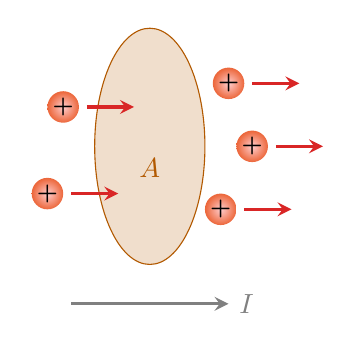
\begin{tikzpicture}[>=stealth]
  \draw[orange!70!black,fill=orange!70!black!20,name=conductor] (0,0) ellipse (0.7 and 1.5) node[below=0.8]{\(A\)};
  \draw[very thick,gray,->] (-1,-2) -- (1,-2) node[right]{\(I\)};

  \foreach \x\y in {-1.1/0.5,-1.3/-0.6,1/0.8,1.3/0,0.9/-0.8} {
    \shade[inner color=white!80!red, outer color=orange!50!red!70!lightgray] (\x,\y) node{\footnotesize\textbf{+}} circle (.2) [radius=1pt];
    \draw[very thick,color=red!70!gray,->] ({\x+0.3},\y) -- ({\x+0.9},\y);
  }

\end{tikzpicture}

  \captionsetup{hypcap=false} % Disable hycap for this fig
  \captionof{figure}{Cargas en movimiento a través de un área \(A\).}
  \label{fig_current}
\end{tcolorbox}
\begin{equation}\label{eq_i_prom}
  I_{\text{prom}} = \frac{\Delta Q}{\Delta t}
\end{equation}

Si la tasa a la que pasan las cargas varía en el tiempo, la corriente instantánea \(I\) se define como:
\[
  I = \lim_{\Delta t \to 0} \frac{\Delta Q}{\Delta t} = \frac{dQ}{dt}
\]
Para que exista un movimiento de cargas, es necesario que exista una fuerza que actúe sobre ellas. Esta fuerza es la fuerza eléctrica o ley de Coulomb, como muestra la ecuación \eqref{eq_coulomb}\footnote{En la ecuación \eqref{eq_coulomb} \(k_e=\qty{8.9876d9}{\newton\metre\squared\per\coulomb\squared}\) es la constante de Coulomb, \(q_1\) y \(q_2\) son las cargas y \(r\) es la distancia entre cargas.},
\begin{equation}\label{eq_coulomb}
  F=k_e \frac{\lvert q_1 \rvert \cdot \lvert q_2 \rvert}{r^2}
\end{equation}
Esta fuerza se manifiesta en un conductor en forma de campo eléctrico \(E\), que actúa sobre las cargas libres (electrones). Al provocar una diferencia de potencial\footnote{La diferencia de potencial es provocada por una f.e.m.}, se crea este campo eléctrico que actúa sobre las cargas libres en el conductor. 

Cuando hay un campo eléctrico en un conductor, las cargas libres se aceleran y adquieren una velocidad. En palabras simples, podemos asociar la corriente eléctrica con el movimiento de cargas libres en un conductor.

En un conductor, los electrones libres se mueven en direcciones aleatorias debido a la temperatura del material. Sin embargo, cuando se aplica un campo eléctrico, estos electrones adquieren una velocidad de arrastre o velocidad de deriva \(v_d\) en sentido opuesto al campo eléctrico. La velocidad de deriva es la velocidad promedio de las cargas (electrones en el caso de un conductor).
\begin{figure}[ht]
  \centering
  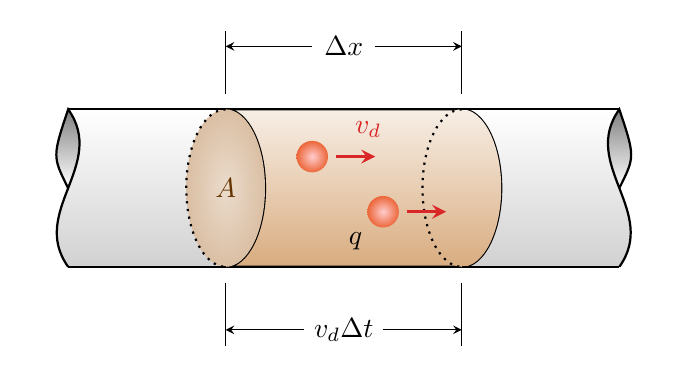
\begin{tikzpicture}[>=stealth]
    \def\rx{0.5}
    \def\ry{1}
    \def\lle{1.5}
    \def\curv{0.5}
    
    % Sombra conductor
    \shade[top color=orange!70!black!10, bottom color=orange!70!black!50] 
      (-\lle, \ry) -- (\lle, \ry)
      arc (90:-90:\rx cm and \ry cm)
      -- (-\lle, -\ry)
      arc (-90:90:\rx cm and \ry cm);

    % Sombra D (de corte)
    \shade (-\lle-2,0) .. controls (-\lle-2+\curv, 0.3) .. (-\lle-2, \ry) .. controls (-\lle-2-\curv+0.3, 0.4) .. (-\lle-2, 0);
    \shade (\lle+2,0) .. controls (\lle+2-\curv, 0.3) .. (\lle+2, \ry) .. controls (\lle+2+\curv-0.3, 0.4) .. (\lle+2, 0);

    % Sombra corte
    \shade[top color=white, bottom color=white!70!black!60] 
      (-\lle,-\ry) -- (-\lle-2,-\ry) .. controls (-\lle-2-\curv, -0.3) and (-\lle-2+\curv, 0.3) .. (-\lle-2, \ry) -- (-\lle,\ry);
    \shade[top color=white, bottom color=white!70!black!60] 
      (\lle,-\ry) -- (\lle+2,-\ry) .. controls (\lle+2+\curv, -0.3) and (\lle+2-\curv, 0.3) .. (\lle+2, \ry) -- (\lle,\ry);

    \draw[thick] 
      (-\lle, \ry) -- (\lle, \ry)
      arc (90:-90:\rx cm and \ry cm)
      -- (-\lle, -\ry)
      arc (-90:90:\rx cm and \ry cm);


    \shade[bottom color=orange!70!black!50, top color=orange!70!black!10] (\lle,0) ellipse (\rx cm and \ry cm);
    \shade[outer color=orange!60!black!36, inner color=orange!60!black!20] (-\lle,0) ellipse (\rx cm and \ry cm);

    % Sección de corte
    \draw[black,thick] (-\lle-2,-\ry) .. controls (-\lle-2-\curv, -0.3) and (-\lle-2+\curv, 0.3) .. (-\lle-2, \ry) .. controls (-\lle-2-\curv+0.3, 0.4) .. (-\lle-2, 0);
    \draw[black,thick] (\lle+2,-\ry) .. controls (\lle+2+\curv, -0.3) and (\lle+2-\curv, 0.3) .. (+\lle+2, \ry) .. controls (\lle+2+\curv-0.3, 0.4) .. (\lle+2, 0);
    \draw[black,thick] (-\lle,\ry) -- (-\lle-2,\ry);
    \draw[black,thick] (-\lle,-\ry) -- (-\lle-2,-\ry);
    \draw[black,thick] (\lle,\ry) -- (\lle+2,\ry);
    \draw[black,thick] (\lle,-\ry) -- (\lle+2,-\ry);

    \draw[thick, dotted] (-\lle,\ry) arc (90:270:\rx cm and \ry cm);
    \draw[thick, dotted] (\lle,\ry) arc (90:270:\rx cm and \ry cm);

    \node at (-\lle, 0) {\color{orange!40!black}\(A\)};

    % Cotas de medida
    \draw[thin] (-\lle,\ry+0.2) -- (-\lle,\ry+1);
    \draw[thin] (\lle,\ry+0.2) -- (\lle,\ry+1);
    \draw[thin,->] (-0.4,\ry+0.8) -- (-\lle,\ry+0.8);
    \draw[thin,->] (0.4,\ry+0.8) -- (\lle,\ry+0.8);
    \node at (0,\ry+0.8) {\(\Delta x\)};

    \draw[thin] (-\lle,-\ry-0.2) -- (-\lle,-\ry-1);
    \draw[thin] (\lle,-\ry-0.2) -- (\lle,-\ry-1);
    \draw[thin,->] (-0.5,-\ry-0.8) -- (-\lle,-\ry-0.8);
    \draw[thin,->] (0.5,-\ry-0.8) -- (\lle,-\ry-0.8);
    \node at (0,-\ry-0.8) {\(v_d \Delta t\)};

    % Cargas
    \shade[inner color=white!80!red, outer color=orange!50!red!70!lightgray] (-0.4,0.4) circle (.2) [radius=1pt];
    \draw[very thick,color=red!70!gray,->] (-0.1,0.4) node[above right=3pt] {\(v_d\)}-- (0.4,0.4) ;
    \shade[inner color=white!80!red, outer color=orange!50!red!70!lightgray] (0.5,-0.3) node[below left=4pt] {\(q\)} circle (.2) [radius=1pt];
    \draw[very thick,color=red!70!gray,->] (0.8,-0.3) -- (1.3,-0.3);
  \end{tikzpicture}
  \caption{Movimiento de cargas en un conductor.}
  \label{fig_movimiento_de_cargas}
\end{figure}


Recordando que \(\Delta Q\) es la cantidad de carga que pasa a través de la sección transversal \(A\), si toma un pedazo de conductor de longitud \(\Delta x\) como se muestra en la figura \ref{fig_movimiento_de_cargas}, puede expresar el volumen de este segmento de conductor como \(A\cdot\Delta x=A\cdot v_d\cdot \Delta t\). Si \(n\) es la densidad de cargas (número de cargas por unidad de volumen), el número de cargas en el segmento es \(nAv_d\Delta t\). Entonces la carga total de esa sección es
\begin{equation}\label{eq_carga_en_el_conductor}
  \Delta Q = (n\, A\, v_d\, \Delta t) q
\end{equation}
donde \(q\) es la carga de cada portador (electrones). Así se puede obtener la expresión de la corriente operando sobre la expresión \eqref{eq_carga_en_el_conductor}. Si divide ambos lados de la ecuación por \(\Delta t\) resulta
\begin{equation}\label{eq_corriente_promedio}
  I_\text{prom}=\frac{\Delta Q}{\Delta t} = n \, A\, v_d\, q
\end{equation}
que es la expresión de la corriente promedio.

\begin{figure}[ht]
  \centering
  \begin{subfigure}[b]{0.48\textwidth}
    \centering
    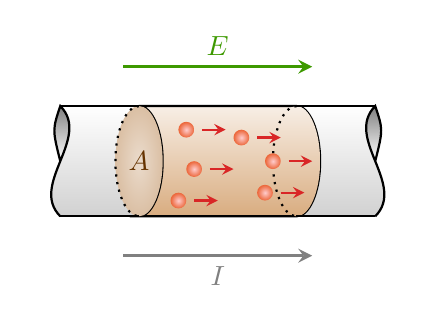
\begin{tikzpicture}[>=stealth]
      \def\rx{0.3}
      \def\ry{0.7}
      \def\lle{1}
      \def\cond{1}
      \def\curv{0.4}
      
      % Sombra conductor
      \shade[top color=orange!70!black!10, bottom color=orange!70!black!50] 
        (-\lle, \ry) -- (\lle, \ry)
        arc (90:-90:\rx cm and \ry cm)
        -- (-\lle, -\ry)
        arc (-90:90:\rx cm and \ry cm);

      % Sombra D (de corte)
      \shade (-\lle-\cond,0) .. controls (-\lle-\cond+\curv, 0.3) .. (-\lle-\cond, \ry) .. controls (-\lle-\cond-\curv+0.3, 0.4) .. (-\lle-\cond, 0);
      \shade (\lle+\cond,0) .. controls (\lle+\cond-\curv, 0.3) .. (\lle+\cond, \ry) .. controls (\lle+\cond+\curv-0.3, 0.4) .. (\lle+\cond, 0);

      % Sombra corte
      \shade[top color=white, bottom color=white!70!black!60] 
        (-\lle,-\ry) -- (-\lle-\cond,-\ry) .. controls (-\lle-\cond-\curv, -0.3) and (-\lle-\cond+\curv, 0.3) .. (-\lle-\cond, \ry) -- (-\lle,\ry);
      \shade[top color=white, bottom color=white!70!black!60] 
        (\lle,-\ry) -- (\lle+\cond,-\ry) .. controls (\lle+\cond+\curv, -0.3) and (\lle+\cond-\curv, 0.3) .. (\lle+\cond, \ry) -- (\lle,\ry);

      \draw[thick] 
        (-\lle, \ry) -- (\lle, \ry)
        arc (90:-90:\rx cm and \ry cm)
        -- (-\lle, -\ry)
        arc (-90:90:\rx cm and \ry cm);


      \shade[bottom color=orange!70!black!50, top color=orange!70!black!10] (\lle,0) ellipse (\rx cm and \ry cm);
      \shade[outer color=orange!60!black!36, inner color=orange!60!black!20] (-\lle,0) ellipse (\rx cm and \ry cm);

      % Sección de corte
      \draw[black,thick] (-\lle-\cond,-\ry) .. controls (-\lle-\cond-\curv, -0.3) and (-\lle-\cond+\curv, 0.3) .. (-\lle-\cond, \ry) .. controls (-\lle-\cond-\curv+0.3, 0.4) .. (-\lle-\cond, 0);
      \draw[black,thick] (\lle+\cond,-\ry) .. controls (\lle+\cond+\curv, -0.3) and (\lle+\cond-\curv, 0.3) .. (+\lle+\cond, \ry) .. controls (\lle+\cond+\curv-0.3, 0.4) .. (\lle+\cond, 0);
      \draw[black,thick] (-\lle,\ry) -- (-\lle-\cond,\ry);
      \draw[black,thick] (-\lle,-\ry) -- (-\lle-\cond,-\ry);
      \draw[black,thick] (\lle,\ry) -- (\lle+\cond,\ry);
      \draw[black,thick] (\lle,-\ry) -- (\lle+\cond,-\ry);

      \draw[thick, dotted] (-\lle,\ry) arc (90:270:\rx cm and \ry cm);
      \draw[thick, dotted] (\lle,\ry) arc (90:270:\rx cm and \ry cm);

      \node at (-\lle, 0) {\color{orange!40!black}\(A\)};

      % Dirección de la corriente convencional
      \draw[very thick, gray, ->] (-\lle-0.2,-\ry-0.5) -- node[below]{\(I\)} (\lle+0.2,-\ry-0.5);
      % Dirección del campo eléctrico
      \draw[very thick, green!60!yellow!60!black, ->] (-\lle-0.2,\ry+0.5) -- node[above]{\(E\)} (\lle+0.2,\ry+0.5);

      % Cargas
      \foreach \x\y in {-0.4/0.4,-0.3/-0.1,-0.5/-0.5,0.3/0.3,0.7/0,0.6/-0.4} {
        \shade[inner color=white!80!red, outer color=orange!50!red!70!lightgray] (\x,\y) circle (.1) [radius=1pt];
        \draw[thick,color=red!70!gray,->] (\x+0.2,\y) -- (\x+0.5,\y) ;
      }
    \end{tikzpicture}
    \caption{Una corriente convencional es tratada como un flujo de cargas positivas, sin importar si las cargas libres del conductor son positivas, negativas o ambas.}
    \label{fig:flujo_de_cargas_positivas}
  \end{subfigure}
  \hfill
  \begin{subfigure}[b]{0.48\textwidth}
    \centering
    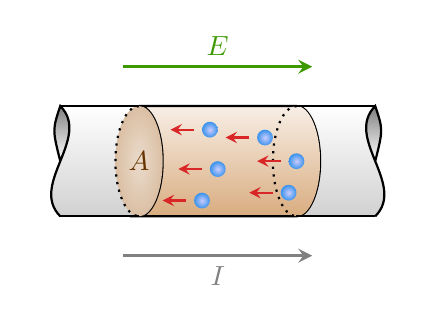
\begin{tikzpicture}[>=stealth]
      \def\rx{0.3}
      \def\ry{0.7}
      \def\lle{1}
      \def\cond{1}
      \def\curv{0.4}
      
      % Sombra conductor
      \shade[top color=orange!70!black!10, bottom color=orange!70!black!50] 
        (-\lle, \ry) -- (\lle, \ry)
        arc (90:-90:\rx cm and \ry cm)
        -- (-\lle, -\ry)
        arc (-90:90:\rx cm and \ry cm);

      % Sombra D (de corte)
      \shade (-\lle-\cond,0) .. controls (-\lle-\cond+\curv, 0.3) .. (-\lle-\cond, \ry) .. controls (-\lle-\cond-\curv+0.3, 0.4) .. (-\lle-\cond, 0);
      \shade (\lle+\cond,0) .. controls (\lle+\cond-\curv, 0.3) .. (\lle+\cond, \ry) .. controls (\lle+\cond+\curv-0.3, 0.4) .. (\lle+\cond, 0);

      % Sombra corte
      \shade[top color=white, bottom color=white!70!black!60] 
        (-\lle,-\ry) -- (-\lle-\cond,-\ry) .. controls (-\lle-\cond-\curv, -0.3) and (-\lle-\cond+\curv, 0.3) .. (-\lle-\cond, \ry) -- (-\lle,\ry);
      \shade[top color=white, bottom color=white!70!black!60] 
        (\lle,-\ry) -- (\lle+\cond,-\ry) .. controls (\lle+\cond+\curv, -0.3) and (\lle+\cond-\curv, 0.3) .. (\lle+\cond, \ry) -- (\lle,\ry);

      \draw[thick] 
        (-\lle, \ry) -- (\lle, \ry)
        arc (90:-90:\rx cm and \ry cm)
        -- (-\lle, -\ry)
        arc (-90:90:\rx cm and \ry cm);


      \shade[bottom color=orange!70!black!50, top color=orange!70!black!10] (\lle,0) ellipse (\rx cm and \ry cm);
      \shade[outer color=orange!60!black!36, inner color=orange!60!black!20] (-\lle,0) ellipse (\rx cm and \ry cm);

      % Sección de corte
      \draw[black,thick] (-\lle-\cond,-\ry) .. controls (-\lle-\cond-\curv, -0.3) and (-\lle-\cond+\curv, 0.3) .. (-\lle-\cond, \ry) .. controls (-\lle-\cond-\curv+0.3, 0.4) .. (-\lle-\cond, 0);
      \draw[black,thick] (\lle+\cond,-\ry) .. controls (\lle+\cond+\curv, -0.3) and (\lle+\cond-\curv, 0.3) .. (+\lle+\cond, \ry) .. controls (\lle+\cond+\curv-0.3, 0.4) .. (\lle+\cond, 0);
      \draw[black,thick] (-\lle,\ry) -- (-\lle-\cond,\ry);
      \draw[black,thick] (-\lle,-\ry) -- (-\lle-\cond,-\ry);
      \draw[black,thick] (\lle,\ry) -- (\lle+\cond,\ry);
      \draw[black,thick] (\lle,-\ry) -- (\lle+\cond,-\ry);

      \draw[thick, dotted] (-\lle,\ry) arc (90:270:\rx cm and \ry cm);
      \draw[thick, dotted] (\lle,\ry) arc (90:270:\rx cm and \ry cm);

      \node at (-\lle, 0) {\color{orange!40!black}\(A\)};

      % Dirección de la corriente convencional
      \draw[very thick, gray, ->] (-\lle-0.2,-\ry-0.5) -- node[below]{\(I\)} (\lle+0.2,-\ry-0.5);
      % Dirección del campo eléctrico
      \draw[very thick, green!60!yellow!60!black, ->] (-\lle-0.2,\ry+0.5) -- node[above]{\(E\)} (\lle+0.2,\ry+0.5);

      % Cargas
      \foreach \x\y in {-0.1/0.4,0/-0.1,-0.2/-0.5,0.6/0.3,1/0,0.9/-0.4} {
        \shade[inner color=white!80!blue, outer color=cyan!50!blue!70!lightgray] (\x,\y) circle (.1) [radius=1pt];
        \draw[thick,color=red!70!gray,->] (\x-0.2,\y) -- (\x-0.5,\y) ;
      }
    \end{tikzpicture}
    \caption{En un conductor metálico, las cargas en movimiento son electrones, pero la corriente aún apunta en la dirección en que fluirían las cargas positivas.}
    \label{fig:flujo_de_cargas_negativas}
  \end{subfigure}
  \caption{Movimiento de cargas en un conductor.}
  \label{fig_corriente_convencional}
\end{figure}


La figura \ref{fig_corriente_convencional} presenta segmentos de material conductor. En la figura \ref{fig:flujo_de_cargas_positivas}, las cargas en movimiento son positivas, la fuerza eléctrica ocurre en la misma dirección que \(E\), y la velocidad de deriva \(v_d\) es de izquierda a derecha. En la figura \ref{fig:flujo_de_cargas_negativas} las cargas son negativas, la fuerza eléctrica es opuesta a \(E\), y la velocidad de deriva \(v_d\) es de derecha a izquierda. Definimos que la corriente, denotada por \(I\), va en la dirección en la que hay un flujo de carga positiva. Por ello, las corrientes se describen como si consistieran por completo en un flujo de cargas positivas, aun en los casos en que se sabe que la corriente real se debe a electrones. Así, en las figuras \ref{fig:flujo_de_cargas_positivas} y \ref{fig:flujo_de_cargas_negativas} la corriente es hacia la derecha. Esta convención sobre la dirección del flujo de la corriente se llama \emph{corriente convencional}. Aunque la dirección de la corriente convencional no es necesariamente la misma en que se desplazan en realidad las partículas con carga, veremos que el signo de las cargas en movimiento tiene poca importancia en el análisis de los circuitos eléctricos.

La ecuación \eqref{eq_corriente_promedio} muestra una expresión para el cálculo de la corriente promedio en un intervalo de tiempo dado. Así, el amperio se deriva de \unit{\coulomb\per\second} (Coulomb por segundo) pero, ¿qué significa esto en términos fundamentales?

Desde la redefinición del SI en 2019, la unidad se basa en valores fijos de constantes naturales. Se fija la carga elemental (la carga de un electrón) exactamente en:
\begin{equation}\label{eq_relacion_coulomb}
    e = \qty{1.602176634d-19}{\coulomb}
\end{equation}

\begin{definition}[Amperio]
  Para comprender la magnitud de un amperio, puede invertir la relación \eqref{eq_relacion_coulomb} para determinar cuántas cargas elementales constituyen un Coulomb:
\begin{align*}
    \qty{1}{\coulomb} &= \frac{1}{1.602176634\times 10^{-19}} ~ e \\
    \qty{1}{\coulomb} &\approx \qty{6.241509d18}{} \text{ cargas elementales}
\end{align*}
Por lo tanto, sustituyendo esto en la definición de corriente (\(I = q/t\)), un amperio queda definido formalmente como:
\begin{equation}
    \qty{1}{\ampere} = \frac{\qty{1}{\coulomb}}{\qty{1}{\second}} \approx \frac{\qty{6.2415d18}{} \text{ electrones}}{\qty{1}{\second}}
\end{equation}
O, dicho de otra forma más fundamental: un amperio es el flujo de aproximadamente \num{6.2415d18} cargas elementales por segundo a través de una sección transversal determinada.
\end{definition}

\subsubsection{Historia de la definición de Amperio}

Es fundamental distinguir entre la definición histórica, que rigió la metrología durante gran parte del siglo XX, y la definición moderna basada en constantes fundamentales.

Anteriormente, el amperio se definía mediante un experimento idealizado de fuerza magnética. Se basaba en la Ley de Ampère para la fuerza entre dos conductores paralelos:
\begin{equation}
    \frac{F}{L} = \frac{\mu_0 I_1 I_2}{2\pi d}
\end{equation}
Para que esta definición fuera válida, el Sistema Internacional fijaba el valor exacto de la permeabilidad magnética del vacío en \(\mu_0 = 4\pi \times10^{-7}\unit{\henry\per\meter}\). Así, si la distancia \(d\) era \qty{1}{\meter} y la fuerza resultante era \qty{2d-7}{\newton} por metro, la corriente se definía como \qty{1}{\ampere}.

Esta definición dependía de una configuración geométrica ideal (cables infinitos, sección despreciable) difícil de replicar con alta precisión en un laboratorio.

La redefinición eliminó la dependencia de la geometría y la fuerza mecánica. Ahora, el amperio se define fijando la carga elemental \(e\) (un contador de partículas) y el segundo (basado en el reloj atómico de cesio).

Al fijar la carga elemental \(e\) como exacta, la permeabilidad del vacío \(\mu_0\) dejó de ser una constante exacta. En el sistema actual, \(\mu_0\) es un valor que debe determinarse experimentalmente, con una incertidumbre asociada (proporcional a la constante de estructura fina \(\theta\)).

\subsection{Definición de Voltio}

Desde el punto de vista de la metrología eléctrica y la teoría de circuitos, el Volt (\unit{\volt}) se define frecuentemente en términos de potencia y corriente, magnitudes que son observables macroscópicamente en un laboratorio.

\begin{definition}[Voltio]
    El Volt es la diferencia de potencial eléctrico entre dos puntos de un conductor que transporta una corriente constante de \qty{1}{\ampere}, cuando la potencia disipada entre estos puntos es igual a \qty{1}{\watt}.
    \[
      U~\unit{\volt} = \frac{P}{I}~\unit{\watt\per\ampere}
    \]
\end{definition}

Esta definición operativa es consistente con la definición conceptual de energía por unidad de carga (\unit{\joule\per\coulomb}). Podemos demostrar esta equivalencia mediante el análisis dimensional, recordando que la potencia (\unit{\watt}) es la tasa de cambio de energía (\unit{\joule\per\second}) y la corriente (\unit{\ampere}) es la tasa de flujo de carga (\unit{\coulomb\per\second}):
\begin{equation}
    \qty{1}{\volt} = \frac{\qty{1}{\watt}}{\qty{1}{\ampere}} = \frac{\qty{1}{\joule\per\second}}{\qty{1}{\coulomb\per\second}} = \frac{\qty{1}{\joule}}{\qty{1}{\coulomb}}
\end{equation}
Por lo tanto, la definición de instrumentación (basada en potencia) y la definición física (basada en trabajo y campo electrostático) son numéricamente y dimensionalmente idénticas.

\subsubsection*{Efecto Josephson}
Como dato adicional, al igual que con el amperio, es importante notar que para mediciones de alta precisión, la definición práctica del volt se realiza actualmente mediante un fenómeno de mecánica cuántica conocido como el Efecto Josephson.

Este efecto relaciona una diferencia de potencial con una frecuencia de radiación \(f\) a través de la constante de Josephson \(K_J\):
\begin{equation}
    V = \frac{f}{K_J} \quad \text{donde} \quad K_J = \frac{2e}{h} \approx \qty{483597.8484}{\giga\hertz\per\volt}
\end{equation}
Donde \(e\) es la carga elemental y \(h\) es la constante de Planck. Este estándar permite calibrar voltímetros con una precisión de hasta una parte en \(10^{10}\), muy superior a la definición basada en la disipación de potencia térmica.

\subsection{Definición de Ohm (Resistencia)}

Mientras que en física la resistencia suele analizarse desde la geometría y las propiedades del material (\(\rho\)), en instrumentación se define de manera operativa basándose en la relación causa-efecto entre tensión y corriente.

\begin{definition}[Resistencia]
    El Ohm (\unit{\ohm}) es la resistencia eléctrica que existe entre dos puntos de un conductor cuando una diferencia de potencial constante de \qty{1}{\volt} aplicada entre estos puntos produce en el conductor una corriente de \qty{1}{\ampere}, siempre que dicho conductor no sea fuente de fuerza electromotriz.
\end{definition}

Esta definición corresponde matemáticamente a la Ley de Ohm macroscópica:
\begin{equation}
    \qty{1}{\ohm} = \frac{\qty{1}{\volt}}{\qty{1}{\ampere}}
\end{equation}

Es crucial notar la condición final de la definición: \textit{``siempre que dicho conductor carezca de fuerza electromotriz''}. En metrología, esto asegura que el objeto medido sea un elemento pasivo puro. Si el componente generara su propio voltaje (como una batería o un termopar activo), la relación \(V/I\) no reflejaría la resistencia óhmica real del material, introduciendo errores de medición sistemáticos.

Aunque el ohm se define por la relación \(V/I\), el \emph{valor} de la resistencia de un componente depende de sus características físicas. Como se detalla en textos de física fundamental, para un conductor óhmico uniforme:
\begin{equation*}
    R = \rho \frac{L}{A}
\end{equation*}
Esta relación es fundamental en el diseño de sensores resistivos (como las galgas extensiométricas o RTDs), donde la medición de \(R\) se utiliza para inferir cambios en la longitud \(L\) o en la resistividad \(\rho\) debidos a la temperatura.

\subsubsection*{Efecto Hall Cuántico}

Para completar la tríada de los estándares eléctricos modernos (junto con el Amperio y el Volt), el patrón primario de resistencia ya no se basa en artefactos de alambre, sino en el Efecto Hall Cuántico.

Este fenómeno ocurre en sistemas de electrones bidimensionales a bajas temperaturas y fuertes campos magnéticos, donde la conductancia se cuantiza. Esto define la constante de von Klitzing (\(R_K\)), que se relaciona con constantes fundamentales:
\begin{equation*}
    R_K = \frac{h}{e^2} \approx \qty{25812.807}{\ohm}
\end{equation*}
Esto permite realizar el ohm con una incertidumbre extremadamente baja, independiente de las propiedades del material del semiconductor usado, basándose únicamente en la constante de Planck (\(h\)) y la carga elemental (\(e\)).

\subsection{Definición de carga eléctrica}

El Coulomb (\(C\)) es la unidad de carga eléctrica. Aunque se ha usado para definir el Amperio, el Coulomb se define como la cantidad de cargas eléctricas elementales (\(e\)) que son transportadas por una corriente de \qty{1}{\ampere} durante un segundo. Es posible definir así al Coulomb ya que, el Sistema Internacional fija la carga elemental y el segundo.

\subsection{Definición Flujo Magnético (Weber)}

Mientras que en el análisis de campos estáticos el flujo magnético se define geométricamente como el producto del campo por el área (\unit{\tesla\meter\squared}), en metrología e instrumentación es más práctico definir la unidad a partir de los efectos de la inducción electromagnética descritos por la Ley de Faraday.\footnote{Recuerde conceptualmente que el flujo magnético \(\Phi_B\) representa la cantidad de líneas de campo magnético que atraviesan un área determinada.}

\begin{definition}[Definición basada en la Inducción]
    El Weber (\unit{\weber}) es el flujo magnético que, al atravesar un circuito de una sola espira y reducirse uniformemente a cero en el intervalo de \qty{1}{\second}, induce en dicho circuito una fuerza electromotriz constante de \qty{1}{\volt}.
\end{definition}

Esta definición operativa se fundamenta en la relación diferencial entre el voltaje inducido \(\mathcal{E}\) y la tasa de cambio del flujo magnético:
\begin{equation}
    |\mathcal{E}| = \left| \frac{d\Phi_B}{dt} \right|
\end{equation}
Si analizamos las unidades de esta ecuación, podemos establecer la equivalencia dimensional entre la definición de ingeniería (voltaje-tiempo) y la definición física (campo-área):
\begin{equation}
    \qty{1}{\volt} = \frac{\qty{1}{\weber}}{\qty{1}{\second}} \implies \boxed{\qty{1}{\weber} = \qty{1}{\volt\second}}
\end{equation}
Esto demuestra que un weber no es más que un voltio-segundo. Esta equivalencia es crucial en instrumentación, ya que los \emph{fluxómetros} modernos no miden el campo magnético directamente, sino que integran el voltaje inducido en una bobina exploradora a lo largo del tiempo:
\[
\Phi_B = \int \mathcal{E} \, dt
\]

\subsubsection*{El Cuanto de Flujo}

Siguiendo la redefinición del SI, el Weber está íntimamente ligado a constantes fundamentales. En sistemas superconductores, el flujo magnético no es continuo, sino que está cuantizado. El cuanto de flujo magnético (\(\Phi_0\)) es una combinación de la constante de Planck y la carga elemental:
\begin{equation}
    \Phi_0 = \frac{h}{2e} \approx \qty{2.067833848d-15}{\weber}
\end{equation}
Esta constante es la inversa exacta de la constante de Josephson (\(K_J\)) utilizada para definir el voltio. Esto cierra el círculo de coherencia metrológica: definimos el Voltio mediante el efecto Josephson y el Segundo mediante el reloj atómico, quedando el Weber automáticamente definido como el producto de ambos.

\subsection{Energía}

El Joule (\unit{\joule}) es la unidad de energía. Partiendo de la potencia \(P\) en relación al trabajo \(w\), la expresión de energía resulta de 
\begin{gather*}
  P=\frac{w}{t}  \quad \text{La potencia es trabajo por unidad de tiempo,}\\
  IV=\frac{w}{t} \quad \implies \quad w=IVt
\end{gather*}
Quedando así definido en función de unidades ya definidas: Amperio, Voltio y segundo.

Por otro lado, el desarrollo de unidades resulta
\[
  \unit{\joule}=\unit{\watt\per\second}=\unit{\volt\ampere\second}
\]

\subsection{Coeficiente de autoinducción (Henry)}

La autoinducción (o inductancia propia) es la medida de la inercia eléctrica de un circuito: su oposición a cualquier cambio en la corriente que fluye a través de él.

\begin{definition}[Definición dinámica del Henry]
  El Henry (\unit{\henry}) se define como la inductancia eléctrica de un circuito cerrado en el que se induce una fuerza electromotriz de \qty{1}{\volt} cuando la corriente que lo recorre varía uniformemente a razón de \qty{1}{\ampere} por segundo.
\end{definition}

Esta definición operativa surge de la relación constitutiva del inductor ideal:
\begin{equation}
  \mathcal{E} = -L \frac{dI}{dt} \implies L = \frac{|\mathcal{E}|}{|dI/dt|}
\end{equation}
Dimensionalmente:
\[
  \qty{1}{\henry} = \frac{\qty{1}{\volt}}{\qty{1}{\ampere\per\second}} = \qty{1}{\volt\second\per\ampere} = \qty{1}{\ohm\second}
\]
Un Henry es un Ohm-segundo. Esto ayuda mucho a entender por qué la inductancia afecta la impedancia en función de la frecuencia.

Alternativamente, desde un punto de vista estático o geométrico, la inductancia representa la capacidad de un circuito para enlazar flujo magnético por unidad de corriente. Si el circuito tiene \(N\) espiras y el flujo magnético a través de cada una es \(\Phi_B\):
\begin{equation}
    L = \frac{N \Phi_B}{I}
\end{equation}
Esta dualidad es importante en instrumentación:
\begin{itemize}
    \item La definición de flujo (\(Wb/A\)) es útil para el diseño de bobinas y transformadores (saturación del núcleo).
    \item La definición de voltaje (\(V \cdot s / A\)) es útil para el análisis de circuitos y la medición de impedancia (\(Z = j\omega L\)).
\end{itemize}
\begin{tcolorbox}[
  colback=red!5!white,colframe=red!75!black!66,title=La Sobretensión Inductiva,breakable
  ]
	Como ha visto, la inductancia \(L\) actúa como una inercia electromagnética. Si intentamos interrumpir instantáneamente la corriente en un circuito altamente inductivo (abriendo un interruptor), la derivada de la corriente respecto al tiempo se vuelve enorme:
	\[
	\frac{dI}{dt} \to -\infty \quad \implies \quad \mathcal{E} = -L \frac{dI}{dt} \to \infty
	\]
	
	Esto provoca que la bobina genere un pico de voltaje transitorio (conocido como \textit{fuerza contra-electromotriz} o \textit{kickback}) que puede alcanzar miles de voltios, mucho mayor que la fuente de alimentación original. Esto puede tener consecuencias en instrumentación:
	\begin{itemize}
		\item Arco eléctrico: Se produce una chispa entre los contactos del interruptor, dañándolos.
		\item Destrucción de equipos: Si hay instrumentos de medición o semiconductores (transistores, microcontroladores) conectados, este pico de tensión puede perforar sus aislamientos y destruirlos instantáneamente.
	\end{itemize}
	
	Para medir o controlar cargas inductivas de forma segura, se coloca un diodo en paralelo con la bobina (polarizado en inversa respecto a la fuente). Cuando se abre el interruptor, la bobina invierte su polaridad y el diodo conduce, permitiendo que la corriente recircule y se disipe suavemente en la resistencia interna de la bobina, evitando el pico de tensión.
\end{tcolorbox}

\subsection{Capacidad eléctrica (Farad)}

Si la autoinducción representa la inercia a la corriente, la capacidad eléctrica representa la \textit{elasticidad} del circuito frente a la tensión. Un capacitor almacena energía en forma de campo eléctrico.

\begin{definition}[Definición estática del Farad]
  El farad (\unit{\farad}) es la capacidad de un conductor eléctrico que, al ser cargado con una carga de \qty{1}{\coulomb}, adquiere un potencial eléctrico de \qty{1}{\volt}.
  \begin{equation}
    C = \frac{Q}{V} \quad \implies \quad \qty{1}{\farad} = \frac{\qty{1}{\coulomb}}{\qty{1}{\volt}}
  \end{equation}
\end{definition}

Esta definición es útil para electrostática, pero en instrumentación y análisis de señales, es más útil la definición dinámica que describe cómo varía el voltaje en el tiempo.

\begin{definition}[Definición dinámica]
  El farad es la capacidad de un circuito en el que, al circular una corriente constante de \qty{1}{\ampere}, la diferencia de potencial entre sus terminales varía a razón de \qty{1}{\volt} por segundo.
\end{definition}

Esta definición surge de la ecuación constitutiva del capacitor ideal:
\begin{equation}
  I = C \frac{dV}{dt} \implies C = \frac{I}{dV/dt}
\end{equation}

Nótese la simetría perfecta con el inductor:
\begin{itemize}
    \item En el inductor, el voltaje depende del cambio de corriente (\(V = L \cdot dI/dt\)).
    \item En el capacitor, la corriente depende del cambio de voltaje (\(I = C \cdot dV/dt\)).
\end{itemize}

Mientras que el valor del farad se define por la relación \(Q/V\), la capacidad física de un componente depende de su construcción. Para un capacitor de placas paralelas:
\begin{equation}
    C = \varepsilon \frac{A}{d}
\end{equation}
Donde \(\varepsilon\) es la permitividad del dieléctrico, \(A\) el área de las placas y \(d\) la distancia entre ellas. En instrumentación, los sensores capacitivos aprovechan esta ecuación: al variar la distancia \(d\) o el dieléctrico, cambia \(C\), permitiendo medir desplazamientos micrométricos o niveles de líquidos.

\begin{tcolorbox}[
    colback=red!5!white,colframe=red!75!black!66,title=La Corriente de Inserción
  ]

Un capacitor se opone a los cambios bruscos de voltaje. Si conectamos un capacitor descargado directamente a una fuente de voltaje (o cortocircuitamos uno cargado), estamos forzando un cambio de tensión instantáneo (\(dt \to 0\)).

Según la ecuación \(I = C \frac{dV}{dt}\), esto demanda una corriente teóricamente infinita. Esto tiene importantes consecuencias en instrumentación:
\begin{itemize}
    \item Chispa y soldadura: Al cortocircuitar un capacitor de gran capacidad, la corriente puede ser de cientos de amperios, fundiendo los contactos del cable.
    \item Daño a fuentes: Al encender un equipo con muchos capacitores, la fuente de alimentación ve un cortocircuito momentáneo que puede activar protecciones o quemar fusibles.
\end{itemize}
\end{tcolorbox}

\subsection{Otras magnitudes derivadas de interés}

Para complementar las unidades fundamentales de tensión, corriente e impedancia, el ingeniero en instrumentación debe estar familiarizado con magnitudes auxiliares que describen propiedades del medio o fenómenos ópticos. A continuación se describen magnitudes adicionales que serán de utilidad.

\subsubsection{Magnitudes Electromagnéticas Adicionales}

\begin{description}
  \item[Conductancia (\(G\))]
  Es el recíproco de la resistencia (\(G = 1/R\)). Mientras la resistencia mide la oposición al flujo, la conductancia mide la facilidad para conducir corriente.
  \[ \qty{1}{\siemens} = \qty{1}{\ampere\per\volt} = \qty{1}{\ohm^{-1}} \]

  \textit{Uso:} Es matemáticamente superior para analizar circuitos en paralelo. Unidad: Siemens (\unit{\siemens}).

  \item[Intensidad de Campo Eléctrico]
  Mide la fuerza que experimentaría una carga unitaria en el espacio o el gradiente de potencial entre dos puntos.

  \textit{Uso:} Fundamental en compatibilidad electromagnética (EMC) para medir ruido irradiado o potencia de antenas. Unidad: Volt por metro (\unit{\volt\per\meter}).

  \item[Inducción Magnética]
  También llamada densidad de flujo magnético. Representa la concentración de líneas de flujo por unidad de área.
  \[ \qty{1}{\tesla} = \qty{1}{\weber\per\meter^2} \]

  \textit{Uso:} Es lo que realmente genera fuerza sobre un cable o induce voltaje en una bobina. Unidad: Tesla (\unit{\tesla}).

  \item[Intensidad de Campo Magnético (\(H\))]
  A diferencia de \(B\) (que depende del material del núcleo), \(H\) depende únicamente de la corriente y la geometría de la bobina externa, sin importar el medio.

  \textit{Uso:} Se utiliza para caracterizar las fuentes de campo magnético independientes del material. Unidad: Ampere por metro (\unit{\ampere\per\meter}).

  \item[Fuerza Magnetomotriz (\(\mathcal{F}\))]
  Es la causa que establece el flujo magnético en un circuito magnético (análogo al voltaje en un circuito eléctrico). Aunque dimensionalmente es corriente (\unit{\ampere}), en ingeniería a menudo se le llama Ampere-vuelta (\unit{A\cdot v}) para denotar que es el producto del número de espiras \(N\) por la corriente \(I\).
  \[ \mathcal{F} = N \cdot I \]
  Unidad: Ampere (\unit{\ampere}).
\end{description}

\subsubsection{Magnitudes Fotométricas}

Es común confundir la potencia de la fuente con la luz recibida. La distinción es vital en diseño de iluminación y sensores ópticos.

\begin{description}
  \item[Flujo Luminoso (\(\Phi_v\))]
  Mide la cantidad total de luz visible emitida por una fuente en todas direcciones. Es la potencia luminosa percibida por el ojo humano. Unidad: Lumen (\unit{\lumen}).

  \textit{Ejemplo:} Una bombilla LED de 10W puede emitir \qty{800}{\lumen}. 

  \item[Iluminancia (\(E_v\))]
  Mide la cantidad de flujo luminoso que incide sobre una superficie específica. Unidad: Lux (\unit{\lux}).
  \[ \qty{1}{\lux} = \qty{1}{\lumen\per\meter^2} \]
  La iluminancia decrece con el cuadrado de la distancia. Así, mientras más lejos este la superficie, menor será la cantidad de iluminación que llegue.
\end{description}

\subsection{Tabla de múltiplos y submúltiplos}

A continuación, la tabla \ref{tab:prefijos_si} muestra algunos de los prefijos utilizados en el sistema internacional.

\begin{table}[ht]
  \centering
  \begin{tabular}{p{0.45\textwidth}p{0.45\textwidth}}
    \toprule
    \textbf{Múltiplos} & \textbf{Submúltiplos} \\
    \midrule
    \textbf{Giga (G)}: \(10^9\) \newline (Mil millones) & \textbf{Mili (m)}: \(10^{-3}\) \newline (Milésima) \\
    \addlinespace
    \textbf{Mega (M)}: \(10^6\) \newline (Un millón) & \textbf{Micro (\(\mu\))}: \(10^{-6}\) \newline (Millonésima) \\
    \addlinespace
    \textbf{Kilo (k)}: \(10^3\) \newline (Mil) & \textbf{Nano (n)}: \(10^{-9}\) \newline (Milmillonésima) \\
    \addlinespace
    & \textbf{Pico (p)}: \(10^{-12}\) \newline (Billonésima) \\
    \bottomrule
  \end{tabular}
  \caption{Prefijos del Sistema Internacional (SI) más utilizados en ingeniería}
  \label{tab:prefijos_si}
  
  \vspace{0.2cm}
  \footnotesize{Para consultar la tabla completa, incluyendo exa, zetta, femto y atto, visite: \\ \url{https://es.wikipedia.org/wiki/Sistema_Internacional_de_Unidades#Tabla_de_m%C3%BAltiplos_y_subm%C3%BAltiplos}}
\end{table}
